\documentclass[12pt]{article}

\usepackage{sbc-template}
\usepackage[utf8]{inputenc}
\usepackage{graphicx,url}
\usepackage{indentfirst}
\usepackage[portuges]{babel}
\usepackage{enumitem}
\usepackage{xcolor}
\usepackage{blindtext}

\sloppy
%---------------------CAPA DO ARTIGO
\title{Reconhecimento Digital de Imagens para Classificação de Personagens}

\author{Gabriel Alexander Teixeira, Luiz Carlos Glomyer, Abraão B. Brandão, Luiz A. Ruiz}

\address{Engenharia de Computação -- Universidade do Estado do Amazonas (UEA)
\\
\email{gaflt.eng17@uea.edu.br, glomyerjunior@hotmail.com, abraaobritof10@gmail.com}
\email{locar.eng17@uea.edu.br}\\
  \\Escola Superior de Tecnologia - EST \\Endereço: Av. Darcy Vargas, 1200 - Parque Dez,\\ Manaus - AM, 69050-020
}
%------------------- FIM DA CAPA & BEGIN{DOCUMENT} = COMEÇO DO DOCUMENTO

\begin{document} 

\maketitle %Comando de Máscara de Capa

%-------------------------INICIO DO RESUMO
\begin{resumo} 
  Este artigo tem como finalidade a aplicação dos conceitos de Ciência de Dados para a identificação de personagens da série de televisão Os Simpsons, mais especificamente os personagens Homer e Bart. Utilizando os conceitos de sistemas de classificação, o objetivo é processar imagens contendo um ou mais personagens e fazer uma extração de dados a fim de usarmos algoritmos de aprendizado de máquina para fazer uma predição de qual(is) são os personagens presentes em uma imagem. Para a criação da proposta foi utilizado o pacote de imagens em bitmap fornecidos pelo professor da disciplina e, como algoritmos-base, os algoritmos de Naive-Bayes e de Árvores de Decisão J48.
\end{resumo}
%---------------------FIM DO RESUMO
%------------------TÓPICO 1
\section{Introdução e apresentação dos softwares a serem utilizados}

A sociedade, com o advento da computação, está se modernizando a cada dia: inúmeras são as inovações criadas para facilitar a vivência ou para automatizar processos, tanto a nível de hardware quanto a nível de software. Porém, ainda existem tarefas que, se fossem usados recursos humanos, se tornariam inviáveis. Diariamente cerca de 97\% dos e-mails enviados na web são spam\cite{SPAM:17}, ou seja, identificar (ou classificar) milhões ou até mesmo bilhões de e-mails seria algo muito custoso. 

Felizmente, com a extensa pesquisa investida no campo de reconhecimento de padrões, nasceu uma subárea chamada Aprendizado de Máquina (ou Machine Learning). Ela consiste em, basicamente, analisar grandes quantidades de dados por meio de algoritmos e "tentar observar" padrões ocultos contidos entre eles, a fim de que seja feita uma predição, que consiste em prever certo atributo, como "sim" ou "não, ou uma classificação, que dado um certo objeto, tente prever em qual categoria ele se encaixa. Neste projeto nós utilizamos o método de classificação para analisar uma imagem dada e, em seguida, nos informar de qual personagem se trata.

Neste projeto usamos os seguintes softwares:

\begin{description}[font=$\bullet$~\normalfont\scshape\color{black!50!black}]

\item[weka] O Weka (Waikato Environment for Knowledge Analysis) é um software que agrega vários algoritmos dedicados ao estudo de aprendizagem de máquina. Ele faz uma análise computacional e estatísticas dos dados fornecidos, recorrendo a diversas técnicas de reconhecimento de padrões para, a partir daí, fazer a classificação ou regressão dos dados.
\\
\item[java] Usamos a linguagem de programação Java para desenvolver a nossa aplicação, utilizando bibliotecas de machine learning, a biblioteca JavaCV para análise de imagens e a API Java Swing para a interface gráfica.
\\
\item[javacv] O JavaCV é uma versão da biblioteca OpenCV para a linguagem de programação Java. Ele oferece várias funcionalidades úteis, como a exibição de imagem em tela cheia acelerada por hardware, métodos fáceis de usar para executar código em paralelo em múltiplos núcleos, calibração geométrica e colorida de câmeras e projetores, detecção e combinação de pontos de recurso, dentre outros.

\end{description}


%------------------TÓPICO 2
\section{Pacote das imagens analisadas}
O pacote de imagens fornecido possui, no total, 293 imagens dos personagens Bart e Homer, sendo 169 imagens do Bart e 124 imagens do Homer. Algumas imagens, no entanto apresentam, apresentam ambos os personagens, o que porventura pode causar uma falha na classificação. Isto nada mais é do que um caso que se encaixa na matriz de confusão presente nos algoritmos de classificação.

 O processamento da imagem é feito por intermédio da análise de incidência de certas tonalidades de cores-chave, ou seja, cada personagem possui alguma cor que o caracteriza: Bart, por exemplo, tem como características principais a cor de sua camisa, a cor de seu calção e a cor de seus sapatos. 
 
 No caso do Homer, a cor branca de sua camisa, que é uma de suas características inerentes, não nos é uma informação útil, pois a cor se confunde com o plano de fundo (background) de todas as imagens presentes no pacote. Essa informação é então devidamente descartada para não ocasionar classificações errôneas, a partir daí tomamos em seu lugar a tonalidade da barba do Homer, a cor de sua calça e a cor de seus sapatos.

%------------------TÓPICO 3
\section{JavaCV e reconhecimento digital de imagens} 

Uma imagem digital é composta, no seu nível mais básico, por um pixel. Um conjunto de pixels forma uma imagem, em um esquema muito semelhante a uma matriz. A cada pixel pode ser atribuída uma cor na escala RGB, partimos então deste princípio para processar as imagens fornecidas. Para o processamento do pacote de imagens foi utilizada a biblioteca JavaCV (Java Computer Vision), uma versão da biblioteca OpenCV portada para a linguagem de programação Java. 

Em suma, a biblioteca busca uma imagem presente em certo diretório do computador e a partir daí faz uma análise da coloração dos pixels, fornecendo porcentagens das cores mais presentes. Trabalhamos com o formato nativo das imagens, o formato bitmap, pois o processo de análise é bastante simplificado e até mesmo reduz a incidência de erros se comparado aos outros formatos de imagem, principalmente pela inexistência dos chamados artefatos de compressão presentes em arquivos do tipo JPG.

%------------------TÓPICO 4
\section{Algoritmo Naive-Bayes}
O algoritmo de Naive-Bayes nada mais é do que uma família de simples classificadores probabilísticos que vêm sendo estudada intensamente desde 1950. É um dos algoritmos mais usados para classificação de texto, sendo aplicado em detecção de spam e até mesmo em diagnósticos médicos. O que caracteriza esse algoritmo e a palavra ingênuo em seu nome (naive) é que ele desconsidera toda e qualquer correlação entre as variáveis \cite{Organica:35}. Ele calcula a probabilidade de um evento ocorrer dado que outro evento já ocorreu.


%--------------------------TÓPICO 5

\section{Algoritmo J48}
Originalmente chamado de C4.5 e ID3, o algoritmo J48 é uma implementação na linguagem de programação Java que deriva destes dois outros algoritmos de árvores de decisão, ambos concebidos originalmente pelo pesquisador Ross Quinlan. O J48 é um algoritmo que ganhou notoriedade após ser publicado em um artigo falando dos 10 melhores algoritmos para mineração de dados, em 2007 \cite{Top:10}. Os seus diferenciais são a contabilidade dos valores perdidos, a podagem de árvores de decisão, a atribuição de valores contínuos dentro de uma variação, dentre outras funcionalidades.

Ele gera árvores de decisão que podem ser usadas para classificação, criando regras a partir das particularidades dos dados analisados. O objetivo é a progressiva generalização de uma árvore de decisão até que ela ganhe equilíbrio de flexibilidade e acurácia \cite{J:48}.


%------------------TÓPICO 6
\section{Implementação do software e análise das imagens}
O software consiste em três pacotes: imagens, OpenCV e interface. No pacote imagens estão todas as imagens presentes no pacote, já no pacote interface estão presentes todas as classes que fazem o intermédio entre a entrada e a saída do programa, tudo de forma gráfica. Essas classes foram desenvolvidas com o auxílio da API Java Swing e da IDE Netbeans.

O pacote onde o real processamento acontece é o pacote OpenCV: nele é gerada a nossa base de dados, no formato arff. Existe uma classe extratora de características, ela recebe uma imagem e, com base nas cores presentes nela, ela retorna as porcentagens de incidência de determinadas cores. Esse é o método-chave para o reconhecimento de nossos personagens. Além de serem extraídas as características, o OpenCV pinta pixel por pixel cada cor que coincide com as cores-chave de um personagem, mostrando como saída a imagem original e a imagem recolorida lado a lado, esta última com apenas com uma única cor nos pontos críticos do personagem.

Após a extração podemos classificar a imagem com base nas porcentagens de cor fornecidas pela classe extratora usando a nossa base de dados anteriormente criada, ou seja, se o personagem em questão se trata do Homer ou se trata do Bart. São utilizados os algoritmos de Naive-Bayes e de árvores de decisão J48, ambos dispostos lado a lado para compararmos a precisão entre um e outro.

\newpage
%-------------------------Conclusão
\section{Conclusão}
Concluímos, assim, que a técnica de reconhecimento de imagens é uma aplicação bem útil de Aprendizado de Máquina, servindo para diversos propósitos. No entanto, esta é uma área extremamente complexa para se trabalhar, os problemas do cotidiano raramente podem ser resumidos por meros padrões de cores, mas sim por formas e formatos, texturas, iluminação, estruturas faciais entre outros quesitos que não são de simples entendimento e implementação. Num escopo simples, entretanto, é uma forma bastante útil de análise de dados, fornecendo resultados satisfatórios.


%--------------------------Referências

\bibliographystyle{plainyr}
\bibliography{Referencia}

\newpage
%---------Figura 1
\begin{figure}[ht]
\centering
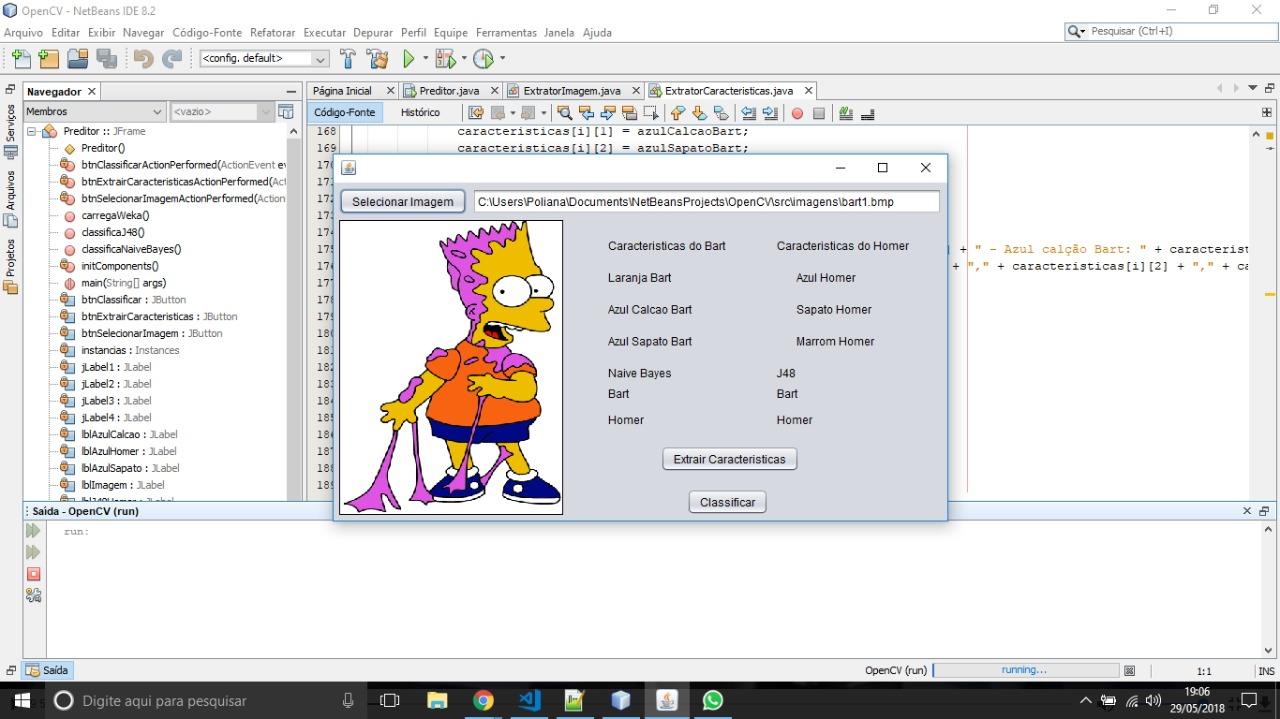
\includegraphics[width=.9\textwidth]{pre-extracao.jpeg}
\caption{Sistemas antes de extrair os dados de uma certa imagem}
\label{fig:exampleFig1}
\end{figure}

%---------Figura 2
\begin{figure}[htt]
\centering
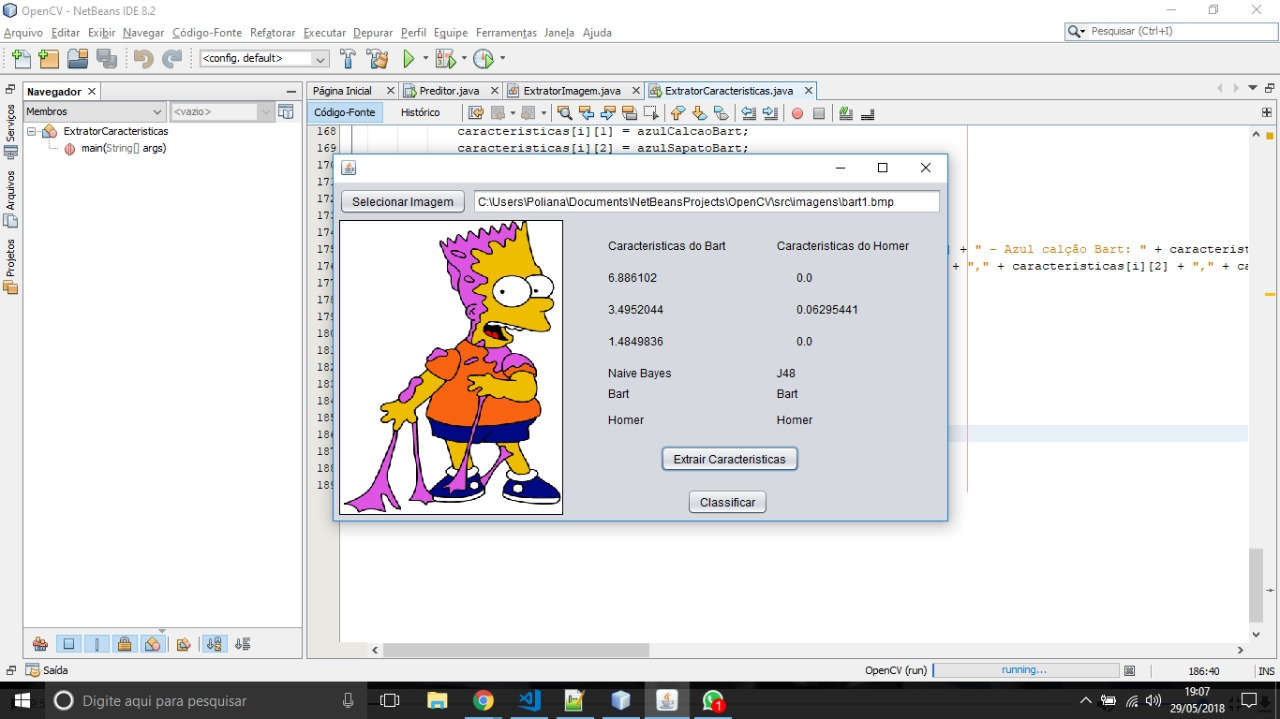
\includegraphics[width=.9\textwidth]{apos-extrair.jpeg}
\caption{Sistema após a extração dos dados da imagem}
\label{fig:exampleFig2}
\end{figure}

%---------Figura 3
\begin{figure}[htt]
\centering
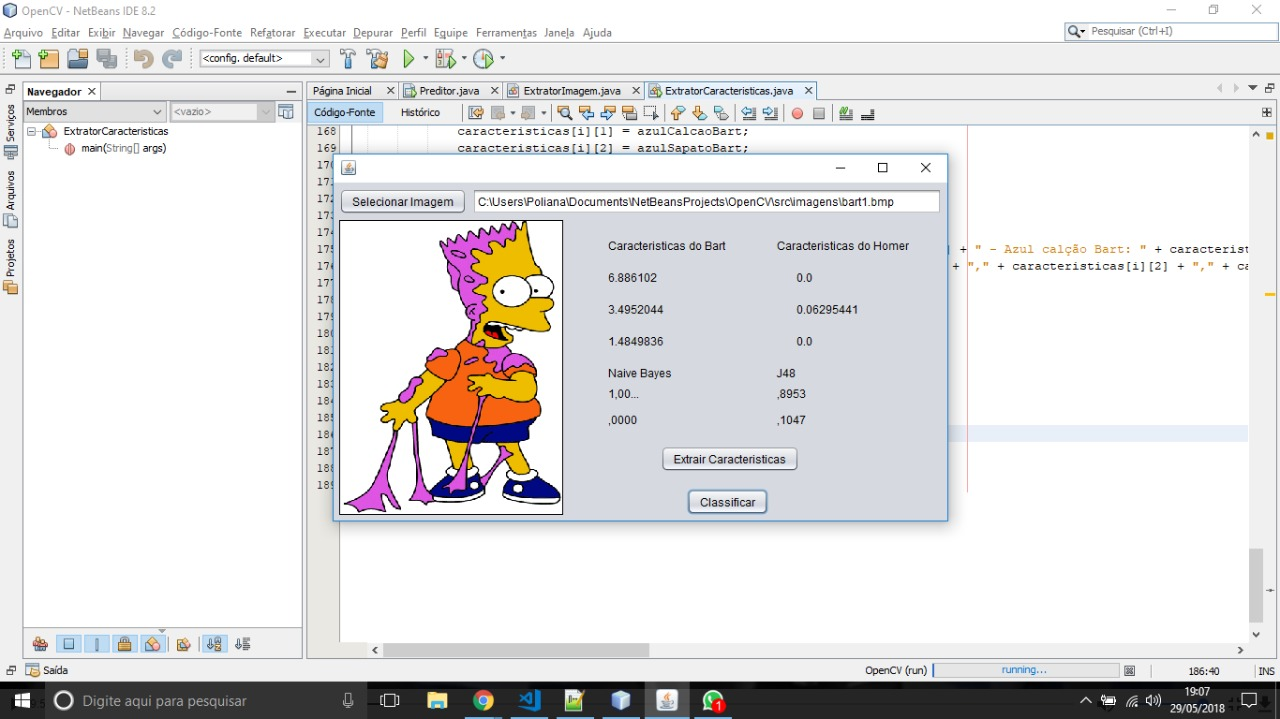
\includegraphics[width=.9\textwidth]{classificacao.jpeg}
\caption{Classificação da imagem com base nos dados extraídos}
\label{fig:exampleFig2}
\end{figure}

%---------Figura 4
\begin{figure}[htt]
\centering
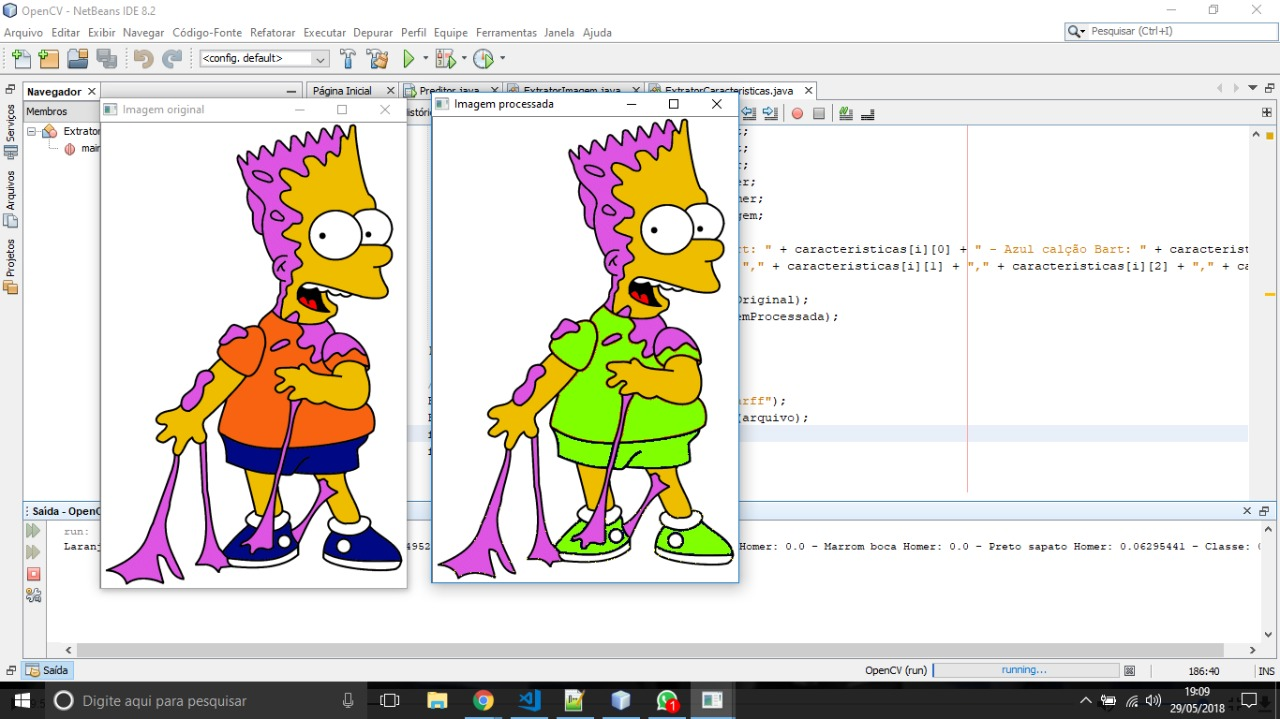
\includegraphics[width=.9\textwidth]{pintura.jpeg}
\caption{Reconhecimento de cor por meio do OpenCV}
\label{fig:exampleFig2}
\end{figure}

%----------------------FIM DOCUMENTO = END{BEGIN}
\end{document}
